\documentclass[11pt]{amsart}

\usepackage{macros, setspace}

\def\U{{\rm U}}
\def\mc{\mathcal}
\def\mcol{\, | \,}
\def\ot{\otimes}
\def\Disj{\operatorname{Disj}}
\def\Open{\operatorname{Open}}
\def\Vect{\operatorname{Vect}}

%trying this out
%\usepackage[upint]{stix}
%\usepackage{cmupint}

\def\brian#1{{\textcolor{blue!65!red}{BRW: {#1}}}}
\def\owen#1{{\textcolor{green!65!black}{OGG: {#1}}}}


\author{Owen Gwilliam and Brian R. Williams}
\date{\today}

\title{Part II}

\spacing{1.25}

\begin{document}
\maketitle


\section{Factorization algebras and quantum field theory}
\label{prefactorization_algebras}

A key idea for us is that much of the content in field theories --- both classical and quantum --- are captured by factorization algebras.
We will introduce that concept now, in the style that sheaves are defined, so first we describe {\em pre}\/factorization algebras and then impose a local-to-global condition to characterize factorization algebras.
With the notion in hand, we will describe several examples and several situations where factorization algebras have already appeared in mathematics and physics, 
albeit in a different formulation.
Finally, we will sketch the main theorem of \cite{CG2}, 
which explains a precise and general relationship between quantum field theories and factorization algebras.

\subsection{The essential idea of a prefactorization algebra}

Let $M$ be a topological space and let $\mc{C}^\otimes$ be a symmetric monoidal category. 
In this paper $M$ is always a smooth manifold (typically a complex manifold) and $\mc{C}$ is ${\rm Vect}$ or ${\rm dgVect}$, with the usual tensor product as the symmetric monoidal product.

A {\em prefactorization algebra} $\cF$ on $M$ taking values in cochain complexes is a rule that assigns a cochain complex $\cF(U)$ to each open set $U \subset M$ along with the following maps and compatibilities.
\begin{itemize}
\item  There is a cochain map $m_V^U: \cF(U) \rightarrow \cF(V)$ for each inclusion $U \subset V$.

\item There is a cochain map $m_V^{U_1,\ldots,U_n} : \cF(U_1) \otimes \cdots \otimes \cF(U_n) \rightarrow \cF(V)$ for every finite collection of open sets where each $U_i \subset V$ and the $U_i$ are pairwise disjoint. The following picture represents the situation.
\begin{center}
 \begin{minipage}[c]{3cm}
 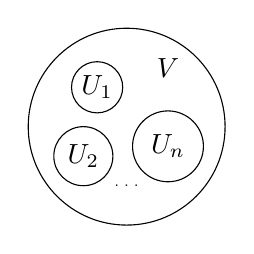
\begin{tikzpicture}[scale=0.25]
 \draw (0,0) circle (5);
 \draw (-1.5,2) circle(1.3) node {$U_1$};
 \draw (-2.2,-1.5) circle (1.5) node {$U_2$};
 \draw (0, -3) node {\tiny$\dots$};
 \draw (2.1,-1) circle (1.8) node {$U_n$};
 \draw (2.1, 3) node {$V$};
 \end{tikzpicture}
 \end{minipage}
\hspace{0.7cm} $\rightsquigarrow$ \hspace{0.5cm}
 \begin{minipage}[c]{8cm}
$\cF(U_1)\otimes\dots\otimes\cF(U_n)\xto{m_V^{U_1,\ldots,U_n}}\cF(V),$
 \end{minipage}
\end{center}

\item The maps are compatible in the obvious way, so that if $U_{i,1}\sqcup\cdots\sqcup U_{i,n_i}\subseteq V_i$ and $V_1\sqcup\cdots\sqcup V_k\subseteq W$, the following diagram commutes.
\begin{center}
\begin{tikzcd}[column sep=small]
{\bigotimes}^{k}_{i=1}{\bigotimes}^{n_i}_{j=1}\cF(U_j) \arrow{dr} \arrow{rr} &   &{\bigotimes}^k_{i=1}\cF(V_i) \arrow{dl}\\
&\cF(W)  &
\end{tikzcd}
\end{center}
\end{itemize}

For an explicit example of the associativity, consider the following picture.
\begin{center}
\hspace{-1cm}
\begin{minipage}{3cm}
{\tiny
\begin{center}
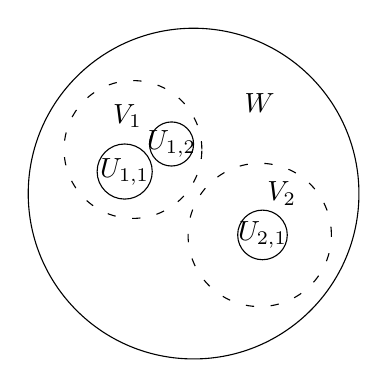
\begin{tikzpicture}[scale=0.35]
 % big circle:
\draw (0,0) circle (6);
\draw (2.4, 3.3) node {$W$};
 % circle V_1:
\draw [style=loosely dashed] (-2.2,1.6) circle (2.5);
\draw (-2.4, 2.8) node {$V_1$};
 % circle V_2:
\draw [style=loosely dashed] (2.4,-1.5) circle (2.6);
\draw (3.2, 0) node {$V_2$};
 % small circles:
\draw (-2.5, 0.8) circle (1) node {$U_{1,1}$};
\draw (-0.8, 1.8) circle (0.8) node {$U_{1,2}$};
\draw (2.5,-1.5) circle (0.9) node {$U_{2,1}$};
%\draw (2.9, -2.1) circle (1.1) node {$U_{2,2}$};
\end{tikzpicture}
\end{center}
}
 \end{minipage}
 \hspace{1.3cm} $\rightsquigarrow$ \hspace{-0.1cm}
\begin{minipage}{8cm}
\begin{tikzcd}[column sep=small]
\cF(U_{1,1}) \otimes \cF(U_{1,2}) \otimes \cF(U_{2,1}) \arrow{dr} \arrow{r}  & \cF(V_1) \otimes \cF(V_2) \arrow{d}\\
&\cF(W) 
\end{tikzcd}
\end{minipage}

The case of $k=n_1=2$, $n_2 = 1$.
\end{center}

This definition bears analogies to familiar objects in mathematics.
On the one hand, $\cF$ resembles a {\em precosheaf}, which is a functor from opens in $M$ to a category like ${\rm Vect}$ or ${\rm dgVect}$.
(A presheaf is a functor out of the opposite category to opens in $M$.) 
Here, however, $\cF$ also assign values to disjoint unions of opens, and it uses the tensor product rather than direct sum.
This feature leads to the other analogy: $\cF$ resembles an algebra, as
the multilinear maps look like multiplications.
These maps let us multiply elements from disjoint regions to get an element in a larger region.

Note that these axioms imply that $\cF(\emptyset)$ is a commutative algebra. 
We say that $\cF$ is a \emph{unital} prefactorization algebra  if $\cF(\emptyset)$ is a unital commutative algebra. In this case, $\cF(U)$ is a pointed cochain complex by the image of the unit $1 \in \cF(\emptyset)$ under the structure map $\cF(\emptyset) \to \cF(U)$. In practice, for our examples, $\cF(\emptyset)$ is $\CC$, $\RR$, $\CC[[\hbar]]$, or $\RR[[\hbar]]$. 

\begin{eg}\label{ex:associativealgebra}
The crucial example to bear in mind is an associative algebra. Every associative algebra $A$ defines a prefactorization algebra $\cF_A$ on $\RR$, as follows. To each open interval $(a,b)$, we set $\cF_A( (a,b) ) = A$. To any open set $U = \coprod_j I_j$, where each $I_j$ is an open interval, we set $\cF(U) = \bigotimes_j A$. The structure maps simply arise from the multiplication map for $A$. Figure ~\ref{fig:assasfact} displays the structure of $\cF_A$. Notice the resemblance to the notion of an $E_1$ or $A_\infty$ algebra. 
%(One takes an infinite tensor products of unital algebras, as follows. Given an infinite set $I$, consider the poset of finite subsets of $I$, ordered by inclusion. For each finite subset $J \subset I$, we can take the tensor product $A^J = \bigotimes_{j \in J} A$. For $J \hookrightarrow J'$, we define a map $A^J \to A^{J'}$ by tensoring with the identity $1 \in A$ for every $j \in J' \backslash J$. Then $A^I$ is the colimit over this poset.) 
~\hfill$\Diamond$
\end{eg}

%\begin{figure}
%\begin{center}
% \begin{minipage}{3cm}
% \begin{tikzpicture}[scale=0.75]
% \begin{scope}[line cap=round,ultra thick]
% \draw (-2.5,0) -- (-1.5,0); 
% \draw (-1,0) -- (-0.5,0); 
% \draw (1,0) -- (2,0); 
% \draw[->,semithick] (0,-0.5) -- (0,-1.5);
% \draw (-2.75,-2) -- (-0.25,-2); 
% \draw (0.75,-2) -- (2.5,-2);  
% \draw[->,semithick] (0,-2.5) -- (0,-3.5);
% \draw (-3,-4) -- (3,-4); 
% \end{scope}
% \end{tikzpicture}
% \end{minipage}
%\hspace{2cm} $\rightsquigarrow$ \hspace{0.5cm}
% \begin{minipage}{8cm}
% \begin{tikzcd}[cramped,column sep=tiny]
%a \otimes b \otimes c \arrow[mapsto]{d} & \in & A \otimes A \otimes A \arrow{d} \\
%ab \otimes c \arrow[mapsto]{d} & \in & A \otimes A \arrow{d} \\
%abc  & \in &A 
%\end{tikzcd}
%\end{minipage}
%\end{center}

\begin{figure}
\begin{center}
 \begin{tikzpicture} 
 \begin{scope}[line cap=round,ultra thick]
 \draw (-2.5,1) -- (-1.5,1); 
 \draw (-1,1) -- (-0.5,1); 
 \draw (1,1) -- (2,1); 
 \draw[->,semithick] (0,0.75) -- (0,0.25);
 \draw (-2.75,-0.1) -- (-0.25,-0.1); 
 \draw (0.75,-0.1) -- (2.5,-0.1);  
 \draw[->,semithick] (0,-0.35) -- (0,-0.85);
 \draw (-3,-1.2) -- (3,-1.2); 
 \end{scope}
 
\node at (4,0) {$\rightsquigarrow$ };

\node at (7,0){
\begin{tikzcd}[cramped,column sep=tiny]
a \otimes b \otimes c \arrow[mapsto]{d} & \in & A \otimes A \otimes A \arrow{d} \\
ab \otimes c \arrow[mapsto]{d} & \in & A \otimes A \arrow{d} \\
abc  & \in &A 
\end{tikzcd}
};
\end{tikzpicture}
\end{center}
\caption{The prefactorization algebra $\cF_A$ of an associative algebra $A$}
\label{fig:assasfact}
\end{figure}

\begin{eg}\label{ex:SymOfCosheaf}
Another important example for us is the symmetric algebra of a precosheaf. 
Let $F$ be a precosheaf of vector spaces on a space $X$. 
For example, consider $F = C^\infty_c$ the compactly supported smooth functions on a manifold. The functor $\cF  = \Sym F: U \mapsto \Sym(F(U))$ defines a precosheaf of commutative algebras, but it also a prefactorization algebra. For instance, if $U$ and $V$ are disjoint opens, we see that
\begin{align*}
\cF(U \sqcup V) = \Sym F(U \sqcup V) & \cong \Sym (F(U) \oplus F(V)) \\ & \cong \Sym(F(U)) \otimes \Sym(F(V)) = \cF(U) \otimes \cF(V),
\end{align*}
and these isomorphisms provide the structure maps for $\cF$.~\hfill$\Diamond$
\end{eg}

We will now sketch another way of phrasing this idea, but the reader who is content with this definition and eager to see examples should feel free to jump ahead, referring back as needed.

\subsection{Prefactorization algebras as algebras over an operad}
\label{sec:disj}

The language of colored operads offers a convenient way to formalize the notion of prefactorization algebra.
A colored operad is a generalization of the idea of a category, where one allows many-to-one maps, and so the term ``multicategory'' is sometimes used. 
See \owen{add citations}

\begin{dfn}
Let $\Disj_M$ denote the following colored operad associated to~$M$: 
\begin{itemize}
\item The colors (or objects) consist of all open subsets of $M$. 
\item For every (possibly empty) finite collection of open sets $\{U_\alpha\}_{\alpha \in A}$ and open set $V$, there is a set of maps $\Disj_M( \{U_\alpha\}_{\alpha \in A} \mcol V)$. If the $U_\alpha$ are pairwise disjoint and all are contained in $V$, then the set of maps is a single point. Otherwise, the set of maps is empty.
\item The composition of maps is defined in the obvious way. 
\end{itemize}
\end{dfn}

\begin{dfn}
Let $\mc{C}$ be a colored operad. 
A \emph{prefactorization algebra}  on $M$ taking values in $\mc{C}$ is a map of colored operads from $\Disj_M$ to~$\mc{C}$. 
\end{dfn}

In other words, a prefactorization algebra \emph{is} an algebra over the colored operad $\Disj_M$.
Since symmetric monoidal categories are special kinds of multicategories, this definition makes sense for symmetric monoidal categories. 

\begin{rmk} 
If $\mc{C}$ is a symmetric monoidal category under coproduct, then a precosheaf on $M$ with values in $\mc{C}$ defines a prefactorization algebra valued in $\mc{C}$. 
Hence, our definition broadens the idea of ``inclusion of open sets leads to inclusion of sections'' by allowing more general monoidal structures to ``combine'' the sections on disjoint open sets.
~\hfill$\Diamond$ 
\end{rmk}

Note that if $\cF$ is any prefactorization algebra, then $\cF(\emptyset)$ is a commutative algebra object of $\mc{C}$. 

\begin{dfn}
We say a prefactorization algebra $\cF$ is \emph{unital} if the commutative algebra $\cF(\emptyset)$ is unital. 
\end{dfn}

\subsection{Encoding ordinary algebras and modules using prefactorization algebras on $\RR$}
\label{AssAsFact}

We explained above how an associative algebra provides a prefactorization algebra on the real line. There are, however, prefactorization algebras on $\RR$ that do {\em not} come from associative algebras. Here we will characterize those that do arise from associative algebras.
 
\begin{dfn}
Let $\cF$ be a prefactorization algebra on $\RR$ taking values in the category of vector spaces (without any grading).   
We say $\cF$ is \emph{locally constant} if the map $\cF(U) \to \cF(V)$ is an isomorphism for any  inclusion of open intervals $U \subset V$. 
\end{dfn}

It is an illuminating exercise to check that this property ensures a prefactorization algebra encodes an associative algebra.

\begin{lem}\label{locally_constant_is_associative}
Let $\cF$ be a locally constant, unital prefactorization algebra on $\RR$ taking values in vector spaces. 
Let $A = \cF(\RR)$. Then $A$ has a natural structure of an associative algebra.  
\end{lem}

One can got further, however, and also capture modules, essentially by marking the line with points.
For simplicity, we will continue to work with ordinary vector spaces with the tensor product as symmetric monoidal structure.

Let $A$ and $B$ be associative algebras and $M$ an $A-B$-bimodule, i.e., $M$ is a left $A$-module and a right $B$-module and these structures are compatible in that $(am)b = a(mb)$ for all $a \in A$, $b \in B$, and $m \in M$. 
We now construct a prefactorization algebra $\cF_M$ on $\RR$ that encodes this bimodule structure. 

Pick a point $p \in \RR$. On the half-line $\{x \in \RR \mid x < p\}$, $\cF_M$ is given by $\cF_A$: to an interval $I = (t_0,t_1)$ with $t_1 <p$, $\cF_M(I) = A$, and the structure map for inclusion of finitely many disjoint intervals into a bigger interval is determined by multiplication in $A$. Likewise, on the half-line $\{x \in \RR \mid p < x\}$, $\cF_M$ is given by $\cF_B$. Intervals containing $p$ are determined, though, by $M$. When we consider an interval $I = (t_0,t_1)$ such that $t_0 < p < t_1$, we set $\cF_M(I)  = M$. The structure maps are also determined by the bimodule structure. For example, given 
\[
s_0 < s_1 < t_0 < p < t_1 < u_0 < u_1,
\]
we have
\begin{align*}
\cF_M((s_0,s_1) \sqcup (t_0, t_1) \sqcup (u_0 , u_1)) 
&= \cF_M((s_0,s_1)) \ot \cF_M((t_0, t_1)) \ot \cF_M((u_0 , u_1)) \\
&= A \ot M \ot B
\end{align*}
and the inclusion of these three intervals into $(s_0,u_1)$ is the map
\[
\begin{array}{ccc}
\cF_M((s_0,s_1)) \ot \cF_M((t_0, t_1)) \ot \cF_M((u_0 , u_1)) & \to & \cF_M((s_0,u_1)) \\
a \ot m \ot b & \mapsto & amb
\end{array}.
\]
The definition of a bimodule ensures that we have a prefactorization algebra. See Figure ~\ref{fig:bimodasfact}.

%\begin{figure}
%\begin{center}
% \begin{minipage}{3cm}
% \begin{tikzpicture}[scale=0.75]
% \begin{scope}[line cap=round,ultra thick]
% \draw (-2.5,0) -- (-1.5,0); 
% \draw (-1,0) -- (0.5,0); 
% \draw[fill=black] (0,0) circle (0.07);
% \draw (1.5,0) -- (2.5,0); 
% \draw[->,semithick] (0,-0.5) -- (0,-1.5);
% \draw (-2.75,-2) -- (0.75,-2); 
% \draw[fill=black] (0,-2) circle (0.07);
% \draw (1.25,-2) -- (2.75,-2);  
% \draw[->,semithick] (0,-2.5) -- (0,-3.5);
% \draw (-3,-4) -- (3,-4);
% \draw[fill=black] (0,-4) circle (0.07); 
% \end{scope}
% \end{tikzpicture}
% \end{minipage}
%\hspace{2cm} $\rightsquigarrow$ \hspace{0.5cm}
% \begin{minipage}{8cm}
% \begin{tikzcd}[cramped,column sep=tiny]
%a \otimes m \otimes b \arrow[mapsto]{d} & \in & A \otimes M \otimes B \arrow{d} \\
%am \otimes b \arrow[mapsto]{d} & \in & M \otimes B \arrow{d} \\
%amb  & \in &M 
%\end{tikzcd}
%\end{minipage}
%\end{center}
%\caption{The prefactorization algebra $\cF_M$ for the $A-B$-bimodule $M$}
%\label{fig:bimodasfact}
%\end{figure}

\begin{figure}
\begin{center}
 \begin{tikzpicture}
 \begin{scope}[line cap=round,ultra thick]
 \draw (-2.5,1) -- (-1.5,1); 
 \draw (-1,1) -- (0.5,1); 
 \draw[fill=black] (0,1) circle (0.07);
 \draw (1.5,1) -- (2.5,1); 
 \draw[->,semithick] (0,0.75) -- (0,0.25);
 \draw (-2.75,-0.1) -- (0.75,-0.1); 
 \draw[fill=black] (0,-0.1) circle (0.07);
 \draw (1.25,-0.1) -- (2.75,-0.1);  
 \draw[->,semithick] (0,-0.35) -- (0,-0.85);
 \draw (-3,-1.2) -- (3,-1.2);
 \draw[fill=black] (0,-1.2) circle (0.07); 
 \end{scope}

\node at (4,0){$\rightsquigarrow$};

\node at (7,0) {
\begin{tikzcd}[cramped,column sep=tiny]
a \otimes m \otimes b \arrow[mapsto]{d} & \in & A \otimes M \otimes B \arrow{d} \\
am \otimes b \arrow[mapsto]{d} & \in & M \otimes B \arrow{d} \\
amb  & \in &M 
\end{tikzcd}
};

\end{tikzpicture}
\end{center}
\caption{The prefactorization algebra $\cF_M$ for the $A-B$-bimodule $M$}
\label{fig:bimodasfact}
\end{figure}

\subsection{Factorization algebras}

We are now in a position to define factorization algebras,
which are prefactorization algebras whose behavior on large open sets is determined by their behavior on small open sets.
To give a precise description, we introduce a Grothendieck topology due to Michael Weiss~\owen{cite  \cite{Weiss} and it is explained nicely and further developed in \cite{BoavidaWeiss}}.

\begin{dfn}
Let $U$ be an open set. A collection of open sets $\mathfrak{U} = \{ U_i \mid i \in I\}$ is a {\em Weiss cover} of $U$ if for any finite collection of points $\{x_1,\ldots,x_k\}$ in $U$, there is an open set $U_i \in \mathfrak{U}$ such that $\{x_1,\ldots,x_k\} \subset U_i$.
\end{dfn}

The Weiss covers define a Grothendieck topology on $\Open(M)$, the poset category of open subsets of a space $M$. We call it the {\em Weiss topology} of~$M$. 

\begin{rmk}
A Weiss cover is certainly a cover in the usual sense, but a Weiss cover typically contains an enormous number of opens. It is a kind of ``exponentiation" of the usual notion of cover, because a Weiss cover is well-suited to studying all configuration spaces of finitely many points in $U$. For instance, given a Weiss cover $\mathfrak{U}$ of $U$, the collection 
\[
\{ U_i^n \mid i \in I\}
\]
provides a cover in the usual sense of $U^n \subset M^n$ for every positive integer~$n$.\hfill$\Diamond$ 
\end{rmk}

\begin{eg}\label{WeissAsExponential}
For a smooth $n$-manifold $M$, there are several simple ways to construct a Weiss cover for $M$. One construction is simply to take the collection of open sets in $M$ diffeomorphic to a disjoint union of finitely many copies of the open $n$-disk. Alternatively, the collection of opens $\{ M \setminus q \mcol q \in M\}$ is a Weiss cover of $M$. One can also produce a Weiss cover of a manifold with countably many elements. Fix a Riemannian metric on $M$. Pick a collection of points $\{q_n\in M \mcol n \in \NN\}$ such that the union of the unit ``discs'' $D_1(q_n) = \{ q \in M \mcol \d(q_n,q) < 1\}$ covers $M$. (Such an open may not be homeomorphic to a disc if the injectivity radius of $q_n$ is less than 1.)  Consider the collection of all ``discs'' $\fD = \{ D_{1/m}(q_n) \mcol m \in \NN, n \in \NN\}$.  The collection of all finite, pairwise disjoint union of elements of $\fD$ is a countable Weiss cover.~\hfill $\Diamond$ 
\end{eg}

Now that we have a notion of cover, we can formulate the local-to-global property for factorization algebras,
which amounts to being a cosheaf for the Weiss topology.
For concreteness' sake, we will continue to have our prefactorization algebras take values in ${\rm dgVect}$,
but it is straightforward to generalize by allowing the values to live in, say, a symmetric monoidal $\infty$-category.

Let us provide the definition of a homotopy cosheaf. 
Let $\Phi$ be a precosheaf on $M$ with values in cochain complexes. Let $\mathfrak{U} = \{U_i \mid i \in I\}$ be a cover of some open subset $U$ of $M$.  Consider the cochain complex with values in cochain complexes whose $-k$th term is 
\[
\bigoplus_{\stackrel{j_0,\ldots, j_k \in I}{j_i \text{ all distinct}}} \Phi (U_{j_0} \cap \cdots \cap U_{j_k}),
\]
and note that this term has an ``internal'' differential arising from $\Phi$. The ``external'' differential is the alternating sum of the structure maps arising from inclusion of $k+1$-fold intersections into $k$-fold intersections. The \emph{\v{C}ech complex of $\mathfrak{U}$ with coefficients in $\Phi$} is the totalization of this double complex:
$$
\check{C}(\mathfrak{U}, \Phi) = \bigoplus_{k=0}^\infty \left( \bigoplus_{\stackrel{j_0,\ldots, j_k \in I}{j_i \text{ all distinct}}} \Phi (U_{j_0} \cap \cdots \cap U_{j_k}) [ k]   \right).
$$
There is a natural map from the $0$th term (of the double complex) to $\Phi(U)$ given by the sum of the structure maps $\Phi(U_i) \to \Phi(U)$. Thus, the \v{C}ech complex possesses a natural map to $\Phi(U)$. We say that $\Phi$ is a \emph{homotopy cosheaf} if the natural map from the \v{C}ech complex to $\Phi(U)$ is a quasi-isomorphism for every open $U \subset M$ and every open cover of $U$. This \v{C}ech complex is simply the dual of the \v{C}ech complex for sheaves of cochain complexes.
In more sophisticated language, the \v{C}ech complex describes the homotopy colimit of $\Phi$ on this simplicial diagram.

We can now define our main object of interest. 

\begin{dfn}
A \emph{factorization algebra} is a prefactorization algebra $\cF$ on $M$ valued in $\Ch$ \owen{change to dgVect?}, with the property that for every open set $U \subset X$ and Weiss cover $\mathfrak{U}$ of $U$, the natural map
$$
\check{C}(\mathfrak{U},\cF) \to \cF(U)
$$
is a quasi-isomorphism. That is, $\cF$ is a homotopy cosheaf with respect to the Weiss topology.
\end{dfn}

We also formulate a multiplicativity condition, as follows. 

\begin{dfn}
A factorization algebra $\cF$ is \emph{multiplicative} if for every pair $U,V$ of disjoint open subsets of $M$, the structure map
$$
\cF(U) \otimes \cF(V) \to \cF(U \sqcup V) 
$$
is a quasi-isomorphism.
\end{dfn}

As verification that this notion has some real content, let's consider a first, interesting case.
We already explained how to produce a locally constant prefactorization algebra $\cF_A$ on $\RR$ from a dg associative algebra $A$.
We could ask about working on the circle $S^1$ instead of $\RR$.
This construction tells us what to assign to every proper open subset of $S^1$: for instance, to each open interval, we assign $A$.
The \v{C}ech complex should then tell us what to assign to the whole circle.
Remarkably, this construction recovers a well-known invariant: the Hochschild chains ${\rm Hoch}_*(A)$ of~$A$.

\begin{thm}[\owen{citations}]
The prefactorization algebra $\cF_A$ extends to a factorization algebra on $S^1$, and
\[
{\rm Hoch}_*(A) \simeq \check{C}(\mathfrak{U},\cF_A)
\]
for any Weiss cover of~$S^1$.
\end{thm}

The reader can check by hand that for an ordinary algebra $A$, the value on the circle is $A/[A,A] = {\rm HH}_0(A)$.
This theorem tells us that factorization homology can be seen as a generalization of Hochschild homology,
where one simultaneously generalizes the circle to an arbitrary closed manifold and an algebra to a factorization algebra.

It can be hard to check whether a given $\cF$ is a homotopy cosheaf, since computing the \v{C}ech complex is typically difficult.
There are some useful abstract results, such as the fact that a factorization algebra is determined by its behavior on a basis for the Weiss topology.
But there is also a rich source of examples in differential geometry, and hence from physics.

Given a vector bundle $E \to M$ (possibly a graded vector bundle), 
let $E^{\boxtimes m} \to M^m$ denote the external product of $E$ with itself $m$ times.
Let $\cE_c(U)$ denote compactly supported sections of $E$ over $U$, 
and similarly let $\cE^{\boxtimes m}_c(U^m)$ denote compactly supported sections of $E^{\boxtimes m}$ over $U^m$.
Let $\Sym^m(\cE_c)(U)$ denote the sections that are invariant under the action of the symmetric group $S_m$ on~$U^m$.
We define a functor $\Sym(\cE_c): \Open(M) \to \Vect$ by
\[
\Sym(\cE_c)(U) = \bigoplus_m \Sym^m(\cE_c)(U),
\]
which is a kind of symmetric algebra on $\cE_c(U)$.
(Those familiar with functional analysis will note that taking sections of the product bundles is a nice way of completing the algebraic tensor product of sections on each component bundle.)
This construction is actually a cosheaf for the Weiss topology, just as $\cE_c$ is a cosheaf for the ordinary topology;
in this sense, the Weiss topology is an ``exponentiation'' of the ordinary topology just as $\Sym(V)$ is an ``exponentiation'' of a vector space~$V$.
We have seen in Example~\ref{ex:SymOfCosheaf} how $\Sym(\cE_c)$ determines a prefactorization algebra,
so the following theorem should be plausible.

\begin{thm}[\owen{cite book}]
For $E \to M$ a graded vector bundle, the functor $\Sym(\cE_c)$ encodes a factorization algebra on $M$.
If we equip $\cE_c$ with a differential operator $d$ of degree 1 suc that $d^2 = 0$ so that $(\cE_c, d)$ is a cosheaf of differential complexes,
then $(\Sym(\cE_c), d)$ is a factorization algebra, where $d$ denotes the natural extension.
\end{thm}

Two examples of differential complexes play a key role in applications: 
\begin{itemize}
\item the de Rham complex $(\Omega^*, d)$ on a smooth manifold, which is relevant for topological field theories, and 
\item the Dolbeault complex $(\Omega^{0,*}, \dbar)$ on a complex manifold, which is relevant for holomorphic field theories.
\end{itemize}
One can take, of course, these complexes with sections in a flat vector bundle (for the de Rham case) or a holomorphic vector bundle (for the Dolbeault case).

\subsection{Algebras over the little disks operad}

Associative algebras are familiar to every mathematician, but as we have just seen, they reflect and encode one-dimensional geometry.
It is then natural to ask about higher-dimensional versions of algebra.
Topologists developed such a systematic generalization, often called $E_n$ algebras or algebras over the little $n$-disks operad,
which we now describe and relate to prefactorization algebras on~$\RR^n$.
In relation to the subject of this paper, we mention that $E_n$ algebras arise naturally from $n$-dimensional topological field theories;
we will soon introduce a holomorphic analog of $E_n$ algebras relevant to holomorphic field theories,
modeled on the discussion here.

Fix a dimension $n$. 
Let $D^n(x,r)$ denote the open disk of radius $r$ centered at $x \in \RR^n$,
and let $D^n$ denote the unit disk~$D^n(0,1)$.

\begin{dfn}
Let $E_n$ denote the colored operad with a single color $D^n$ and a topological space $E_n(k)$ of maps from $k$ copies of $D^n$ to itself given by configurations of $k$ disjoint disks:
\[
E_n(k) = \left\{ \begin{matrix}(x_1, \ldots, x_k) \in (D^n(0,1))^k,\\ (r_1, \ldots, r_k) \in (0,1)^k\end{matrix} \,\bigg|\, \text{\begin{tabular}{c}the disks $D^n(x_i,r_i)$ are pairwise disjoint\\ but each contained in the unit disk $D^n$\end{tabular}}\right\}.
\]
\end{dfn}

When $n = 1$, the operad encodes the idea of associative multiplication:
we get pictures much like those we drew earlier with intervals, 
except that now we can slide and stretch the intervals because we have a space of operations.
More accurately, $E_1$ is a model for associative algebras up to homotopy; 
it is closely related to the $A_\infty$ operad. \owen{Let me check how people compare these.}

For arbitrary $n$, this definition encodes concretely the idea of $n$ directions of multiplication.
If one fixes a direction, such as a coordinate axis, and works with disks lined up in this direction,
one sees an $E_1$ structure.

\owen{Add picture? We drew 2d pictures earlier.}

An algebra over this operad is called an $E_n$-algebra.
A classic example from topology is given by taking the $n$-fold based loop space
\[
\Omega^n_x(X) = \{ \gamma: \overline{D^n} \to X \mcol \gamma(\partial \overline{D^n}) = x\}
\]
of a based space $(X,x)$ (i.e., a topological space with a distinguished point) and $\overline{D^n}$ denotes the closed unit $n$-disk.
Maps that send the boundary of a disk to the base point can be extended naturally to bigger disks: just send the rest of the big disk to the basepoint.
\owen{Should I spell out the structure of the algebra?}
Examples include \owen{What to mention?}

Factorization algebras on $\RR^n$ and $E_n$ algebras should be closely related,
as can be seen by drawing pictures of the configurations of disks that control operations.

\begin{dfn}
A factorization algebra $\cF$ on an $n$-manifold $M$ is \emph{locally constant} if for each inclusion of open disks $D \subset D'$, then the map $\cF(D) \to \cF(D')$ is a quasi-isomorphism.
\end{dfn}

For $M = \RR$, we have already discussed how locally constant factorization algebras relate to associative algebras, starting with Example~\ref{ex:associativealgebra}.
Lurie has shown the following vast extension of this example. (See section 5.4.5 of \cite{LurieHA}, particularly Theorem 5.4.5.9.)

\begin{thm}\label{thm:locisen}
There is an equivalence of $(\infty,1)$-categories between $E_n$ algebras and locally constant factorization algebras on~$\RR^n$.  
\end{thm}  

We remark that Lurie and Ayala-Francis uses a different gluing axiom than we do. A careful comparison of the different axioms and a proof of their equivalence (for locally constant factorization algebras) can be found in \cite{Matsuoka}. We emphasize that higher categories are necessary for a rigorous development of these constructions and comparisons, although we will not emphasize that point in our discussion below, which is expository in nature.

\begin{rmk}
This theorem, together with our work in these two books, builds an explicit bridge between topology and physics. Topological field theories in the physicist's sense, such as perturbative Chern-Simons theory, produce locally constant factorization algebras, which can then be viewed as $E_n$ algebras and analyzed using the powerful machinery of modern homotopy theory. Conversely, intuition from physics about the behavior of topological field theories suggests novel constructions and examples to topology. Much of the amazing resonance between operads, homological algebra, and string-theoretic physics over the last few decades can be understood from this perspective.~\hfill $\Diamond$
\end{rmk}

\begin{rmk}
We have shown how thinking about prefactorization algebras on a real line ``decorated'' with points (i.e., with a kind of stratification) reflects familiar algebraic objects like bimodules. By moving into higher dimensions and allowing more interesting submanifolds and stratifications, one generalizes this familiar algebra into new, largely-unexplored directions. See \cite{AyalaFrancisTanaka} for an extensive development of these ideas in the setting of locally constant factorization algebras.
~\hfill $\Diamond$
\end{rmk}

\subsection{How factorization algebras appear in QFT}

In \cite{CG1, CG2} a systematic relationship is provided between field theories and factorization algebras.
The slogan is 
\begin{quote}
the observables of a field theory living on a manifold $M$ form a factorization algebra on~$M$. 
\end{quote}
To make a mathematical statement, one needs to be precise about what a field theory is.
From hereon, whenever we speak of a classical or quantum field theory, we will mean the definitions articulated in \cite{CosBook,CG1, CG2}, which encompass the Euclidean versions of many field theories studied in physics and mathematics.
Those books use the Batalin-Vilkovisky (BV) formalism for quantization, a homological method generalizing the BRST approach and widely regarded as the most powerful and general way to quantize gauge theories. 

\begin{thm}
\label{main}
The observables of a classical field theory on $M$ form a factorization algebra $\Obs^{cl}$ that assigns to every open set, a 1-shifted Poisson algebra (i.e., a commutative dg algebra equipped with a Poisson bracket of cohomological degree one). A BV quantization of this theory yields a factorization algebra $\Obs^q$ that is a flat deformation of $\Obs^{cl}$ over~$\RR[[\hbar]]$.
\end{thm}

This theorem provides an elegant interpretation of BV quantization as a kind of deformation quantization. In the setting of mechanics (or one-dimensional field theory, since a particle has a worldline), deformation quantization explains the transition from classical to quantum as deforming the observables from a Poisson algebra to an associative algebra. 
This theorem allows one to interpret quantization of field theories---on manifolds of arbitrary dimension---as a deformation quantization from a 1-shifted Poisson factorization algebra to a plain factorization algebra. 

In \cite{CG1}, there are several examples of this formalism in action:
\begin{itemize}
\item Basic examples from quantum mechanics, such as the harmonic oscillator, and it is shown how to recover the Weyl algebra and the Hamiltonians from factorization algebras living on~$\RR$. 
\item Scalar field theory on $\RR^n$, where it is shown how the usual correlation functions are encoded in the factorization algebra on~$\RR^n$ and how canonical quantization appears via pushforward of factorization algebras.
\item The free $\beta\gamma$ system on $\CC$---a basic example of a chiral conformal field theory---is constructed and its usual vertex algebra is extracted from the factorization algebra.
\item Abelian Chern-Simons theory, where it is shown how dimensional reduction along a closed surface $\Sigma$ produces the Weyl algebra on the symplectic vector space $H^1(\Sigma)$ and how line operators form a (very simple!) braided monoidal category.
\end{itemize}
These examples, while not complicated, exhibit in detail how factorization algebras provide a bridge from action functionals to algebra in a broad sense. 

This formalism has shown its power in a number of nontrivial applications:
\begin{itemize}
\item Grady, Li, and Li \cite{GLL} give a direct connection between Fedosov quantization and the factorization algebra of a 1-dimensional field theory.
%\item Gorbounov, Williams and I \cite{GGW} constructed rigorously a 2-dimensional QFT depending on a Calabi-Yau manifold $X$, known as the curved $\beta\gamma$ system, and showed the factorization algebra recovers the chiral differential operators of~$X$.
\item Li and Li \cite{LiLi} constructed the topological B-model and show the factorization algebra recovers the expected topological vertex algebra (see \cite{LiVOA} for a deeper treatment).
\item Costello, Francis, and Gwilliam \cite{CFG} have shown how the factorization algebra of Chern-Simons theory for $\fg$ encodes a quantum group $U_\hbar \fg$ over~$\CC[[\hbar]]$.
\item Rabinovich \cite{RabAxial} showed how the local index theorem and the axial anomaly are simultaneously captured by quantizing free fermions (associated to Dirac operators). Subsequently, he recovered the Quillen determinant line~\cite{RabDet}.
\item Costello \cite{CosYangian} introduced a 4-dimensional gauge theory whose factorization algebra recovers the Yangian,
and subsequently gave extensive applications to quantum integrable systems with Witten and Yamazaki \cite{CWY1,CWY2, CY}.
\end{itemize}
There are others, connected with central topics such as mirror symmetry and the AdS/CFT correspondence, 
and we will discuss holomorphic field theories extensively below.

Thanks to the efforts of people who have adopted this BV/factorization framework,
we now also understand its connection to many important structural aspects of QFT, 
such as asymptotic freedom \cite{EWY}, current algebras \cite{GWcurr}, the Anderson-Higgs mechanism \cite{EG}, and the CS/WZW correspondence~\cite{GRW, CosDimGai}.
In each case this enriched mathematical language offers a new and (we would argue) clarifying point of view.
In turn, physics offers new vistas or rich applications for mathematicians to explore.

\subsection{Chiral conformal field theories and vertex algebras}

\owen{I want to discuss how VOAs relate to factorization algebras, notably our CDO project, Si's results, and Brueggeman's thesis. We should also gesture at the Beilinson-Drinfeld approach.}

\end{document}
